\section{ProgC}

    \subsection{Wichtige Kurzbefehle}
		\begin{tabular}{ll}
			\verb|cd "Path"| & Pfad anwählen \\
			\verb|cd ..| & um eine Ebene nach oben (zurück) \\
			\verb|mkdir "Ordnername"| & Ordner erstellen \\
			\verb|rmkdir "Ordnername"| & Ordner löschen \\
			\verb|rm -rf *| & Alles innerhalb vom aktuellen Ordner löschen \\
			\verb|rm "Datei"| & Datei löschen \\
			\verb|mv "Name alt" "Name neu"| & Datei umbenennen \\
			\verb|cp "Datei alt" "Datei neu"| & Datei kopieren und benennen \\
			\verb|clang -Wall -o "Outputname" "Inputdatei"| & clang-Compiler mit Warnungen \\
			\verb|clang -Wall -o "Outputname" "Inputdatei" -lm| & -lm für Mathebibliothek \\
			\verb|ls| & Listet alle Files im akt. Verzeichnis auf \\
			\verb|ls -l| & Inkl. Informationen wie Grösse u.a. \\
			\verb|ls -a| & Inkl. versteckten Dateien \\
			\verb|ls -al| & Beide Varianten \\
		\end{tabular}

	\subsection{Zahlensysteme}
		\begin{tabular}{|l|l|l|l|l|l|l|l|}
			\hline
			$2^0$ = 1 & $2^1$ = 2 & $2^2$ = 4 & $2^3$ = 8 & $2^4$ = 16 & $2^5$ = 32 & $2^6$ = 64 & $2^7$ = 128 \\
			\hline
		\end{tabular}

		\begin{tabular}{|l|l|l|l|}
			\hline
			\textbf{Grösse} & \textbf{Abk.} & \textbf{Genauer Wert} & \textbf{Näherung} \\
			\hline
			Kilobyte & kB & $2^{10}$ = 1024 Bytes & $10^3$ Bytes \\
			\hline
			Megabyte & MB & $2^{20}$ = 1 048 576 Bytes & $10^6$ Bytes \\
			\hline
			Gigabyte & GB & $2^{30}$ = 1 073 741 824 Bytes & $10^9$ Bytes \\
			\hline
			Terabyte & TB & $2^{40}$ = 1 099 511 627 776 Bytes & $10^12$ Bytes \\ 
			\hline
		\end{tabular}

		\begin{tabular}{|l|llllll|}
			\hline
			Oktal & 3 Bits & $X_8$ & $X_O$ & $X_q$ & $X_oct$ & $0X$ \\
			\hline
			Hex & 4 Bits   & $X_16$ & $X_h$ & $XH$ & $X_hex$ & 0xX \\
			\hline
		\end{tabular}

		\paragraph{Hexadezimal}
			\begin{tabular}{llllllllllllllll}
				0 & 1 & 2 & 3 & 4 & 5 & 6 & 7 & 8 & 9 & 10 & 11 & 12 & 13 & 14 & 15 \\
				0 & 1 & 2 & 3 & 4 & 5 & 6 & 7 & 8 & 9 & A & B & C & D & E & F \\
			\end{tabular}
			
		\paragraph{ASCII (7-Bit)}
			
			Ordnet gängigen Schriftzeichen einen Zahlenwert zu, um diese in einem Digitalrechner präsentieren zu können.
			Die Tabelle ist wichtig, um für geg. Schriftzeichen den in der Maschine repräsentierten Zahlenwert zu ermitteln (und umgekehrt).

			Nachfolger: Unicode (8-, 16-, 32-Bit)
	
	\subsection{Datentypen}
		\subsubsection{Datentypen}
			\begin{tabular}{lccll}
				\textit{Typ} & \textit{Anz. Bytes} & \textit{Bereich} & \textit{printf} & \textit{Spezielles} \\
				\hline
				\textbf{Ganze Zahlen} & & & & \\
				byte & 1  & 0 ... +255 & & \\
				short & 2 & $-2^{15} ... +2^{15}-1$ & \verb|%d; %i| & Hex: \verb|%x; %X| \\
				int & 4 & $-2^{31} ... +2^{31}-1$ & \verb|%d| & Hex: \verb|%x; %X| \\
				long & 8  & $-2^{63} ... +2^{63}-1$ & \verb|%ld; %li| & Hex: \verb|%x; %X| \\
				\hline
				\textbf{Dezimalzahlen} & & & (Expon.: \verb|%e|) & \\
				float  & 4  & $1.2E-38$ ... $3.4E+38$ & \verb|%f| & 6 Dez.stellen \\ %6 dez
				double & 8  & $2.3E-308$ ... $1.7E+308$ & \verb|%lf| & 15 Dez.stellen \\ %15 dez
				\hline
				\textbf{Spezial} & & & & \\
				char    & 1 & Einzelne Buchstaben & \verb|%c| & \\
				boolean & 1 & True / False & & \\
				string  &   & Zeichenkette; Text & \verb|%s| & \\
				\hline
				\textbf{Vorzeichen, Versch.} & & & & \\
				unsigned char          & 1 & 0 ... +255    & \verb|%c| & \\
				signed char            & 1 & -128 ... +127 & \verb|%c| & \\
				unsigned int           & 4 & 0 ... $+2^{32}-1$ & \verb|%u| & \\
				short int              & 2 & $-2^{15} ... +2^{15}-1$ & \verb|%hd| & \\
				unsigned short int     & 2 & 0 ... $+2^{16}-1$ & \verb|%hu| & \\
				long int               & 4 & $-2^{31} ... +2^{31}-1$ & \verb|%ld| & \\
				unsigned long int      & 4 & 0 ... $+2^{32}-1$ & \verb|%lu| & \\
				long long int          & 8 & $-2^{63} ... +2^{63}-1$ & \verb|%lld| & \\
				unsigned long long int & 8 & 0 ... $+2^{64}-1$ & \verb|%llu| & \\
				long double            & 16 & $3.3E-4932$ ... $1.1E+4932$ & \verb|%Lf| & 18 Dez.stellen \\ %18 dez
			\end{tabular}
			
 			\textbf{Ganzzahlen} können überlaufen!

			\textbf{Gleitpunktzahlen} haben meist Rundungsfehler. Nie auf Gleichheit prüfen!

			\textbf{Wertebereich:} \\
			\begin{tabular}{lll}
				$\cdot$ unsigned & 0...$(2^n-1)$               & n=8 : 0...255 \\
				$\cdot$ signed   & $-2^{n-1}...+(2^{n-1}-1)$ & n=8 : -128...+127 \\
			\end{tabular}
			\\
			\textbf{Stellenbreite:} \verb|%7.2f| $\rightarrow$ \verb*|    .  |, \verb|%4d| $\rightarrow$ \verb*|    |(res. immer 4 Zahlenbreiten)

		\subsubsection{Typumwandlung}
			\verb|float f = 41.7;|\\
			Implizit: Eine Kommazahl ohne \verb|f| am Ende hat den Typ \verb|double|
			\\
			\\
			\verb|int x = (int) f;|\\
			Explizit: x hat den Wert 41, Nachkommastellen werden abgeschnitten

		\subsubsection{Namen}
			\begin{minipage}{0.35\linewidth}
				\begin{itemize}
					\item Buchstaben a-z, A-Z
					\item Ziffern 0-9
					\item Underscore
					\item \verb|alpha| $\neq$ \verb|Alpha|
				\end{itemize}
				\textbf{Das erste Zeichen darf keine Ziffer sein}
			\end{minipage}
			\hfill
			\begin{minipage}{0.6\linewidth}
				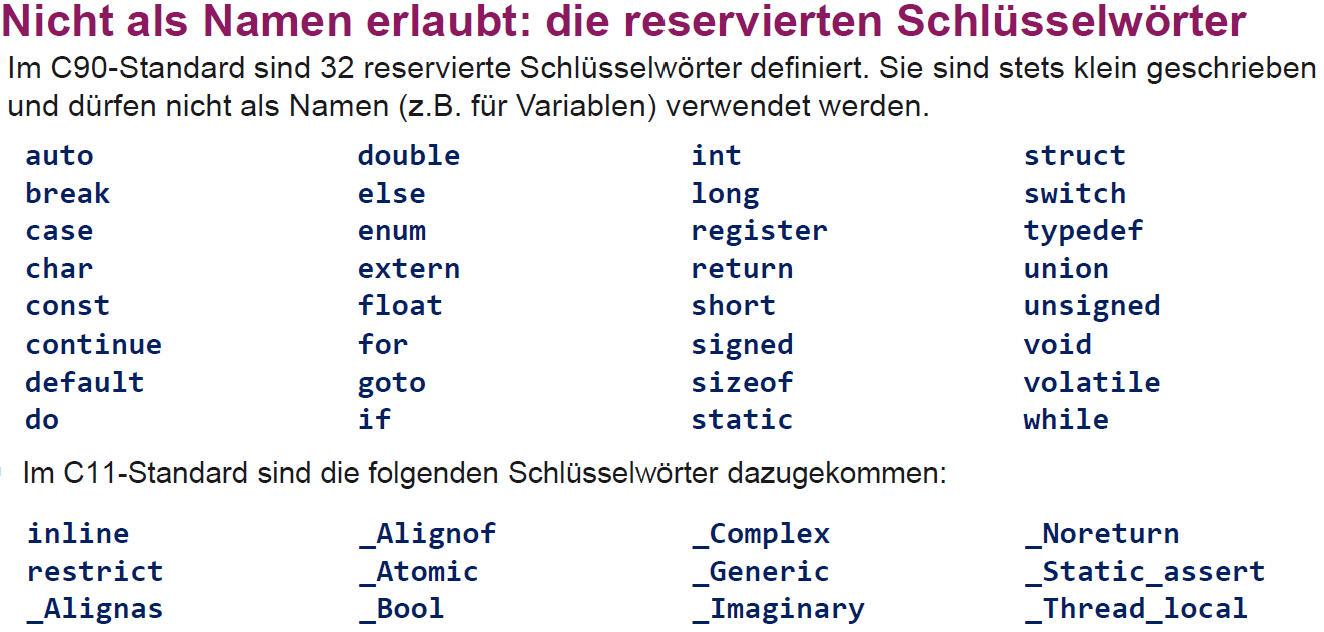
\includegraphics[width=1\linewidth]{Bilder/verbotene_namen.png}
			\end{minipage}

		\subsubsection{Konstanten}
			\begin{minipage}{0.45\linewidth}
				Literale Konstanten:\\
				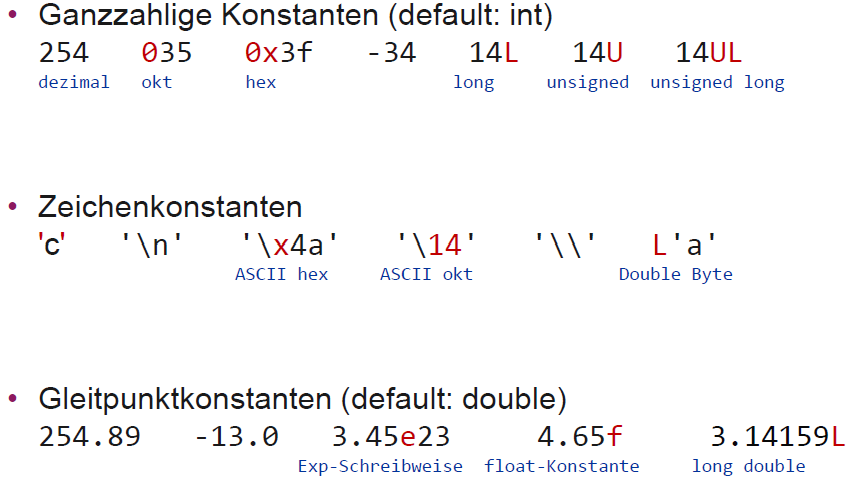
\includegraphics[width=1\linewidth]{Bilder/lit-konstanten.png}
			\end{minipage}
			\hfill
			\begin{minipage}{0.45\linewidth}
				Symbolische Konstanten:
				\begin{lstlisting}[language=C]
//Mit #define
#define PI (3.14159)

//Mit enum
enum{
	listLength = 40;
	commLength = 30;
	dateLength = 20;
}
				\end{lstlisting}
			\end{minipage}

	\subsection{Variablen}
		\begin{minipage}{1\linewidth}
			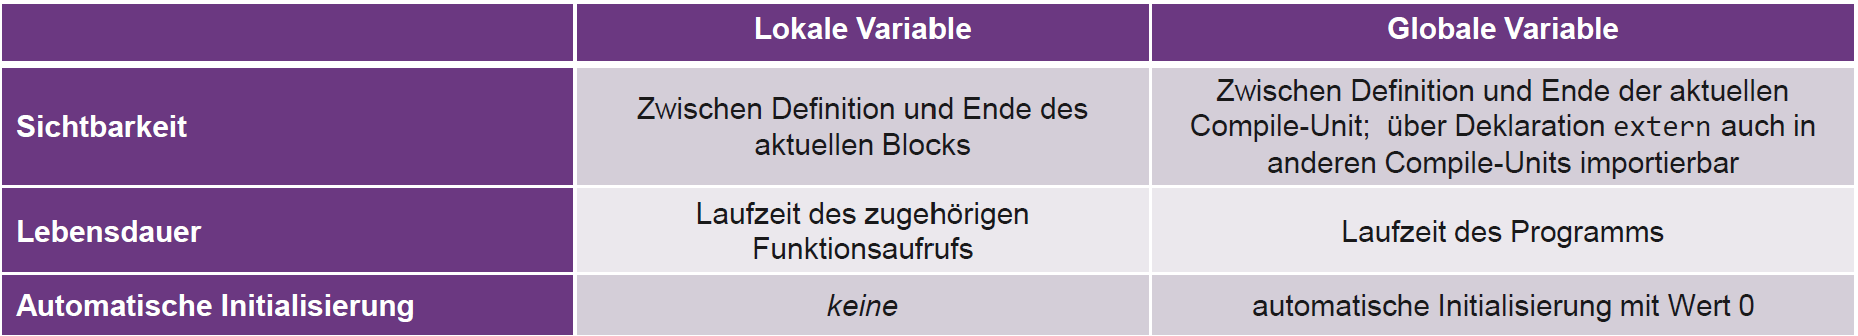
\includegraphics[width=1\linewidth]{Bilder/sichtbarkeit_variablen.png}
		\end{minipage}

	\subsection{Operatoren und Operanden}
		\begin{itemize}
			\item unär (monadisch): hat einen einzigen Operator
			\begin{itemize}
				\item Inkremental ++
				\item De-, Referenzieren (\&, *)
				\item !wahrheitswert (Negation)
			\end{itemize}
			\item binär (dyadisch): hat zwei Operanden
			\begin{itemize}
				\item z.B. 3+4 od. a+b
			\end{itemize}
			\item ternär (triadisch): hat drei Operanden
			\begin{itemize}
				\item \textbf{Mini-If}: \verb|wahrheitswert?wert1:wert2|\\
				(wert1 für \textit{wahr}, wert2 für \textit{falsch}) \\
				(z.B. \verb|x?"wahr":"unwahr"|)
			\end{itemize}
		\end{itemize}

		\subsubsection{Modulo}
			\verb|%| gibt den Restwert einer Rechnung aus\\
			\verb|10 % 3 = 1, 20 % 7 = 6|

		\subsubsection{Priorität \& Assoziativität}
			\begin{minipage}{0.8\linewidth}
					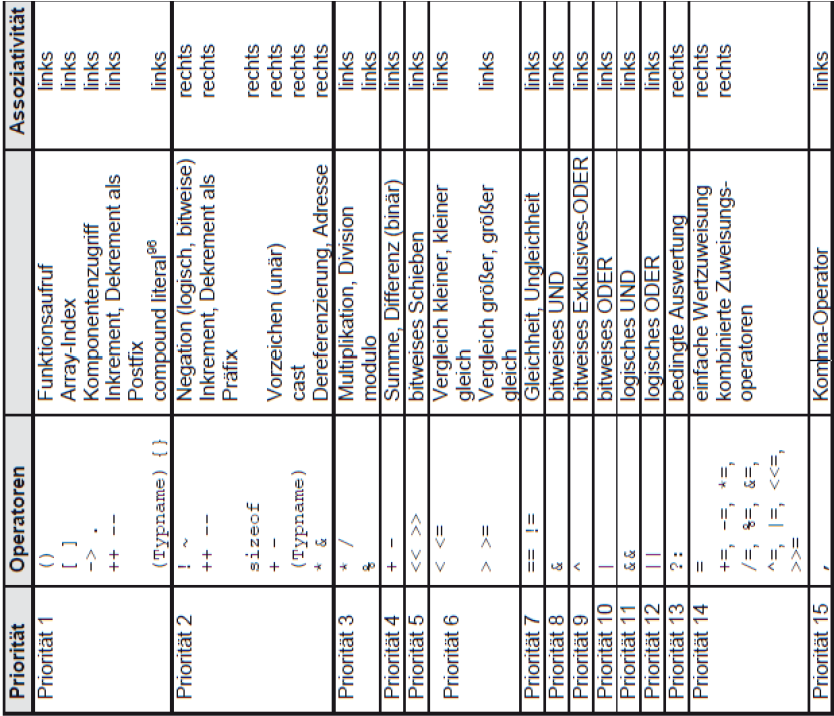
\includegraphics[width=1\linewidth]{Bilder/operatoren_prio.png}
			\end{minipage}
			
			Assoziativität: Reihenfolge der Operationen bei gleicher Priorität
		
		\subsubsection{Inkrementieren \& Dekrementieren}
			\textbf{Postinkrement:}
			\begin{lstlisting}[language=C]
printf("%d", i++)
//i wird zuerst geschrieben, anschliessend inkrementiert
			\end{lstlisting}
			\textbf{Präinkrement:}
			\begin{lstlisting}[language=C]
printf("%d", ++i)
//i wird zuerst inkrementiert, anschliessend geschrieben
			\end{lstlisting}

		\subsubsection{Logisch vs. bitweise Operatoren}
			$\parallel$ = OR\\
			\&\& = AND \\
			\\
			\textbf{Logisch:}
				\begin{lstlisting}[language=C]
signed char a = 0;   //bedeutet unwahr
signed char b = -27; //bedeutet wahr
if(a&&b){
	printf("A und B sind wahr");
}	
				\end{lstlisting}
			\textbf{Bitweise:}
				\begin{lstlisting}[language=C]
unsigned char a = 128: // 1000'0000
unsigned char b = 16;  // 0001'0000
printf("%d\n", a | b); // 1001'0000 
				\end{lstlisting}

	\subsection{Schleifen}
		\subsubsection{For-Schleife}
			\begin{minipage}{.7\linewidth}
				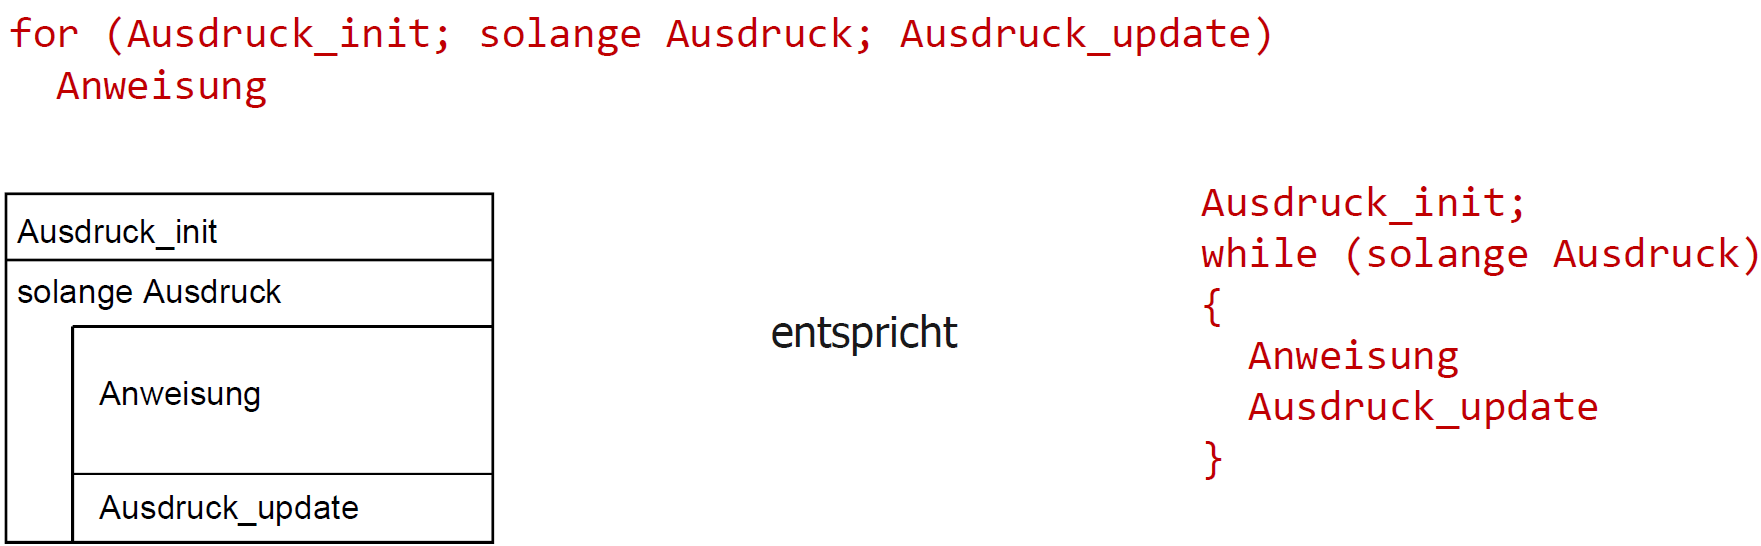
\includegraphics[width=0.95\linewidth]{Bilder/forschleife.png}
			\end{minipage}
			\hfill
			\begin{minipage}{0.3\linewidth}
				Für Zählschleifen, bzw. wenn die Anzahl Durchläufe bekannt ist
			\end{minipage}

		\subsubsection{Switch-Schleife}
			\begin{minipage}{.6\linewidth}
				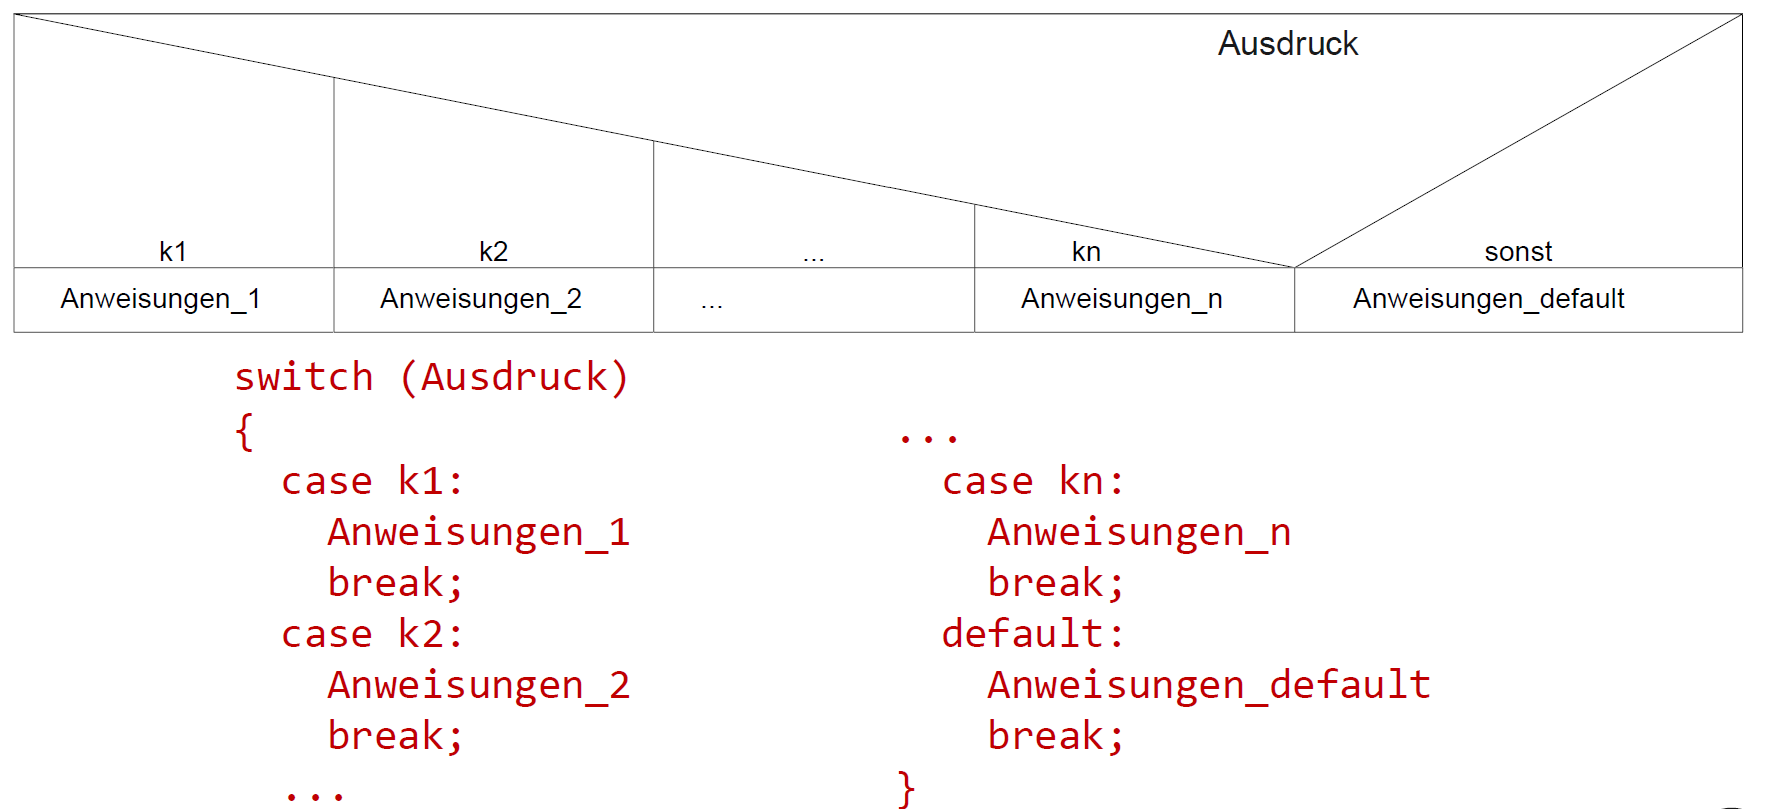
\includegraphics[width=0.95\linewidth]{Bilder/Switch.png}
			\end{minipage}
			\hfill
			\begin{minipage}{.4\linewidth}
				Für Anwendungen, wo eine Überprüfung mehrere Cases haben kann, z.B. Abfrage eines Zustandes (Standby, Off, Idle, Run, ...)
			\end{minipage}

		\subsubsection{Do-While-Schleife}
			\begin{minipage}{.7\linewidth}
				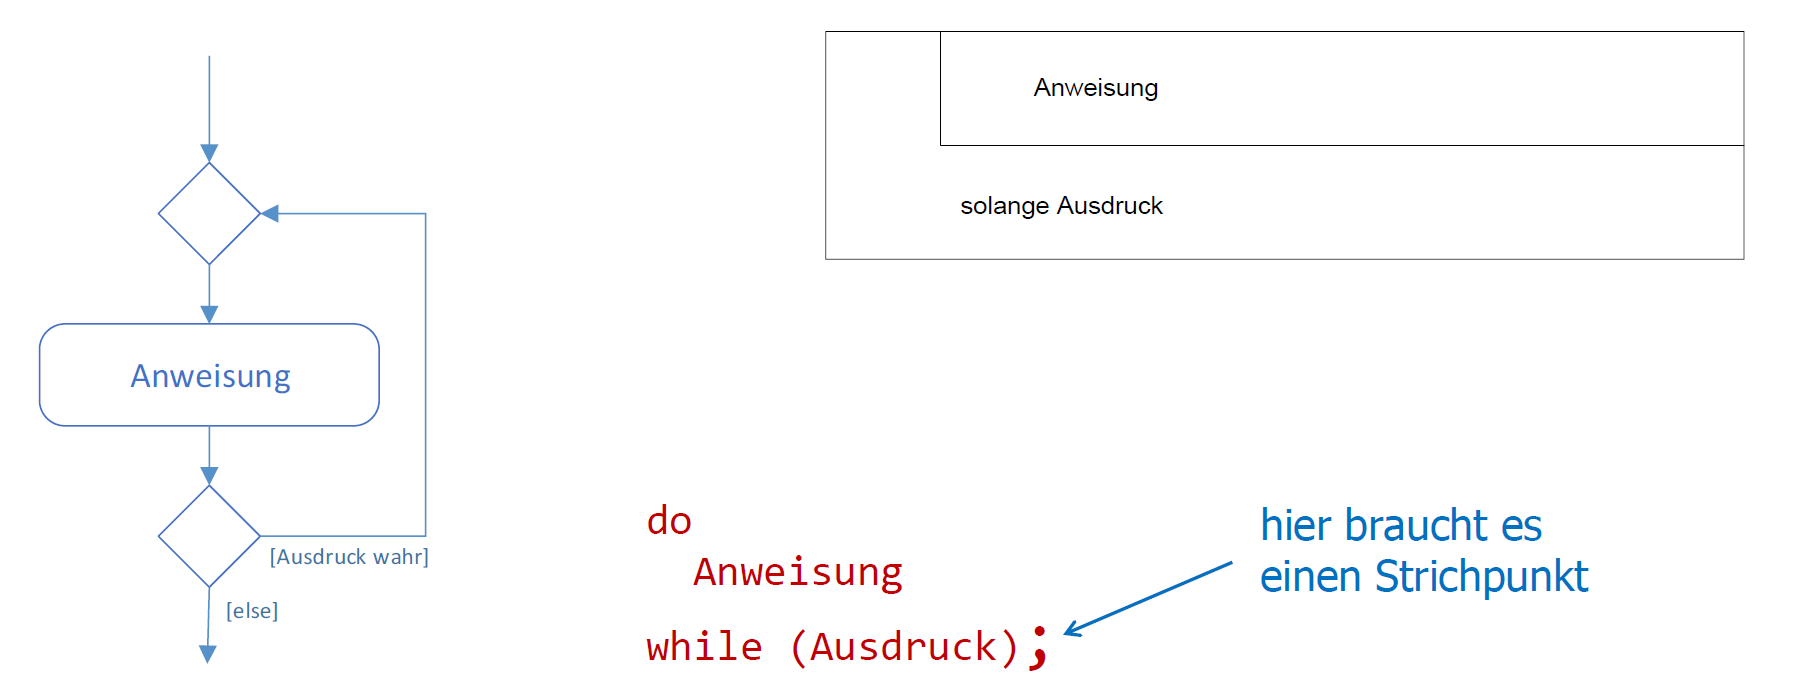
\includegraphics[width=0.95\linewidth]{Bilder/dowhile.png}
			\end{minipage}
			\hfill
			\begin{minipage}{.3\linewidth}
				Keine Zählschleife, das Programm führt min. 1 Durchlauf aus und arbeitet solange Ausdruck = true
			\end{minipage}

		\subsubsection{While-Schleife}
			\begin{minipage}{.45\linewidth}
				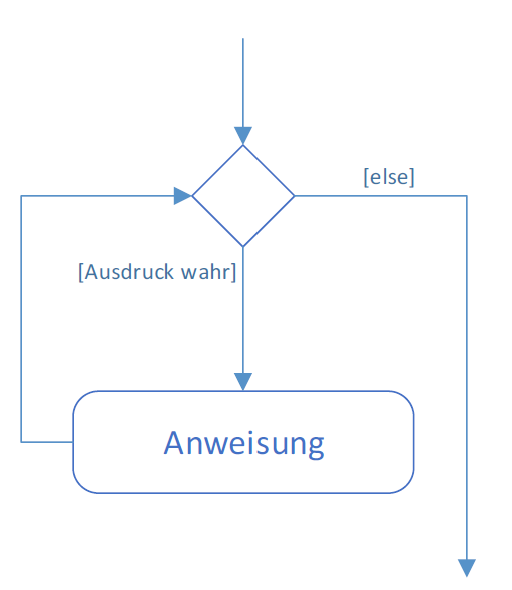
\includegraphics[width=0.5\linewidth]{Bilder/while1.png}
				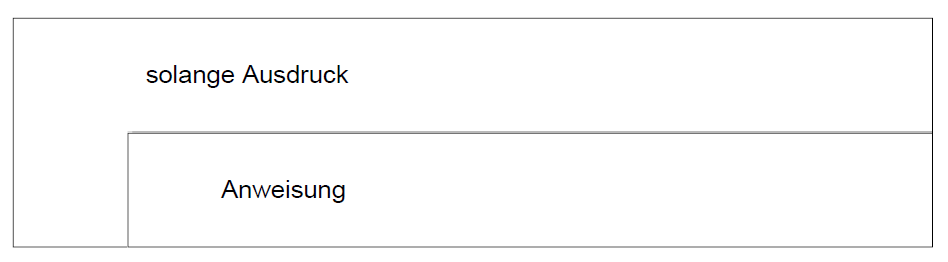
\includegraphics[width=0.5\linewidth]{Bilder/while2.png}
			\end{minipage}
			\hfill
			\begin{minipage}{.5\linewidth}
				Für alle anderen Fälle. Spezialfall: \verb|while(1)| ist ein konstanter Loop im Programm
			\end{minipage}

		\subsubsection{Sprunganweisungen}
			\begin{itemize}
				\item \verb|break|: Schleifen abbrechen, zurückhaltend einsetzen!
				\item \verb|continue|: nächsten Schleifendurchgang starten, sehr zurückhaltend einsetzen!
				\item \verb|return|: aus Funktion zum Aufruf springen
				\item \verb|goto|: zu einer Marke springen, VERMEIDEN!
			\end{itemize}

	\subsection{Pointer}
		\subsubsection{Nullpointer}
			\begin{minipage}{1\linewidth}
				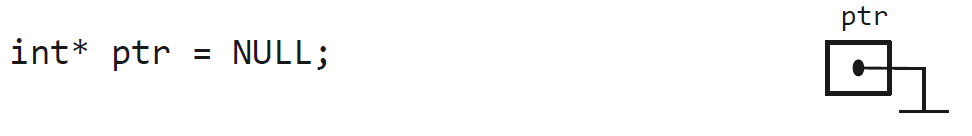
\includegraphics[width=0.95\linewidth]{Bilder/nullpointer.png}
			\end{minipage}

		\subsubsection{Ref- und Dereferenzieren}
			\begin{tabular}{l|l}
				\textbf{Referenzieren} & \textbf{Dereferenzieren} \\
				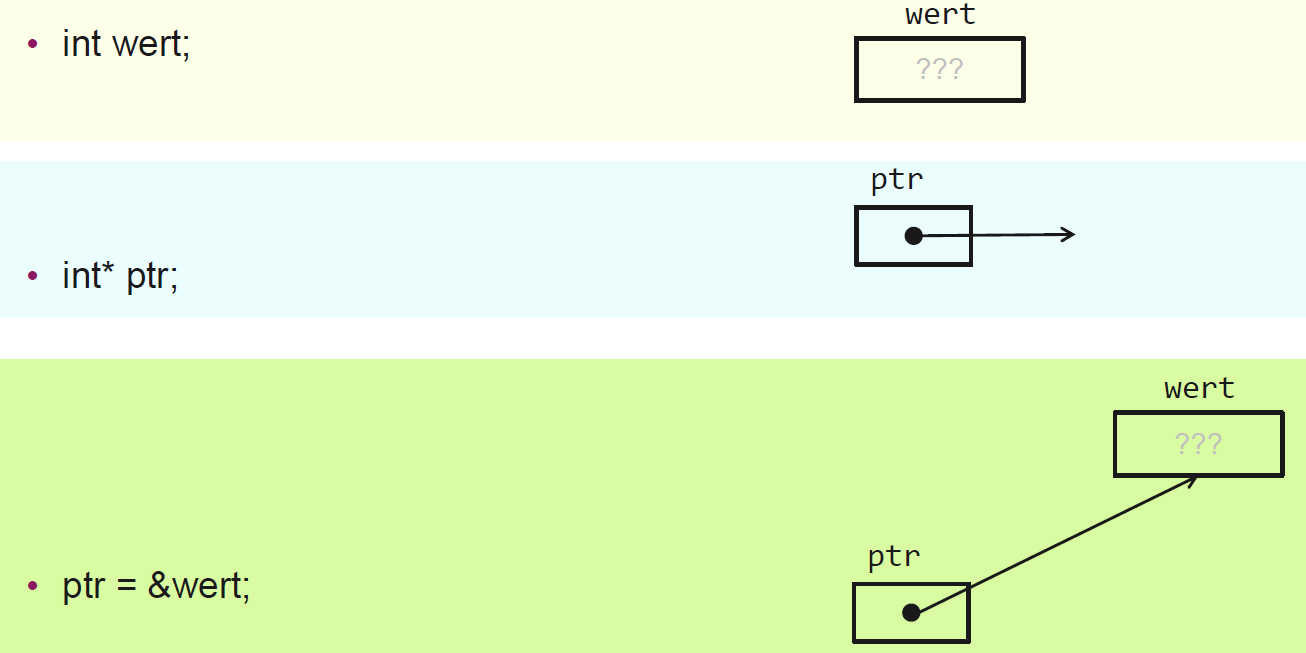
\includegraphics[height=3.2cm]{Bilder/referenzieren.png} &  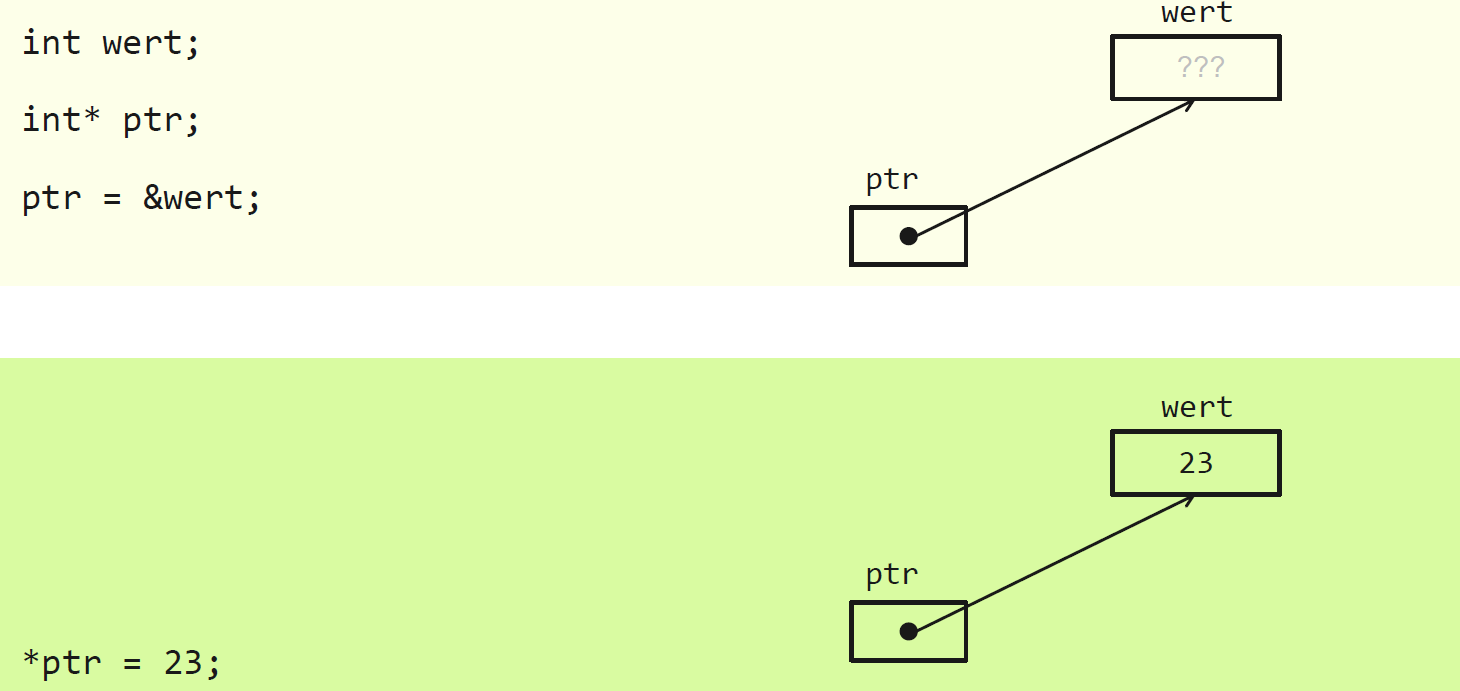
\includegraphics[height=3.2cm]{Bilder/dereferenzieren.png} \\
				\textbf{\&} verknüpft den Pointer mit einer Variable   &  \textbf{*} liefert den Inhalt der Speicherzelle der Adr. \\
			\end{tabular}

			\begin{minipage}{1\linewidth}
				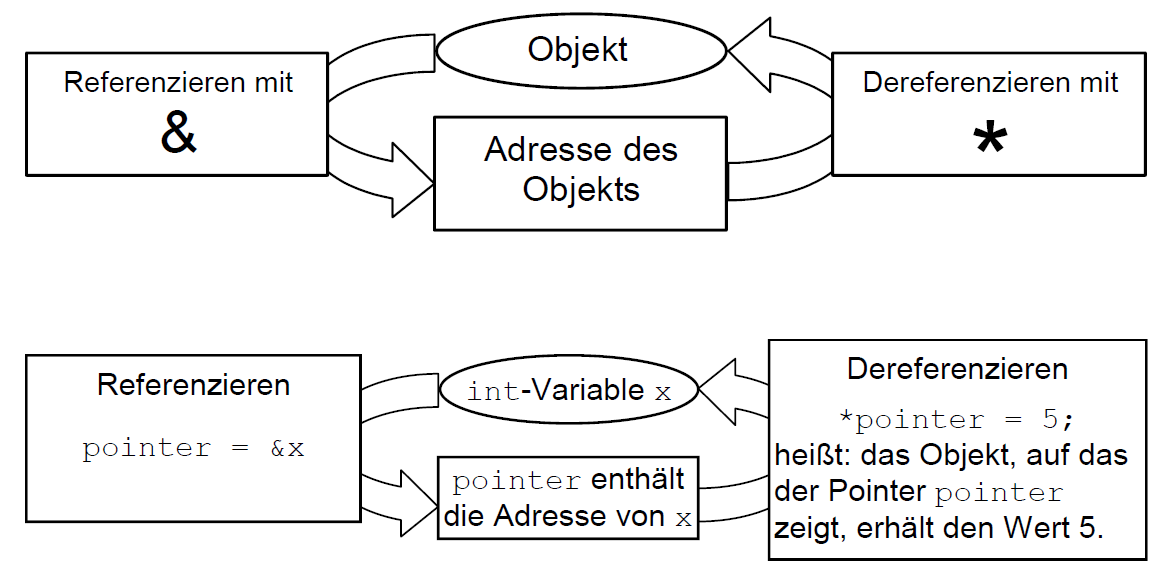
\includegraphics[width=0.5\linewidth]{Bilder/vergl-ref-deref.png}
			\end{minipage}

			%ToDo: Prüfungsbeispiel reinpappen

		\subsubsection{Zuweisungen}
			\begin{lstlisting}[language=C]
int     a;
double  d;
int*    pi = &a;
int*    pj;
double* pd = &d;
void*   pv; 

pv = pd;	 //erlaubt, da pv void-Pointer
pj = pi;	 //erlaubt, gleicher Typ
pd = pi;	 //nicht erlaubt, untersch. Typen
pi = pv;	 //erlaubt, da pv void-Pointer
pd = (double*)pj;//erlaubt da Type-Cast
			\end{lstlisting}
		
		\subsubsection{Addition, Subtraktion}
			Von einem Pointer können ganze Zahlen addiert oder subtrahiert werden. Der Pointer \textbf{ptr} bewegt sich bei \textbf{ptr$+$n} immer um \textbf{n * sizeof(Typ)} Bytes. \\
			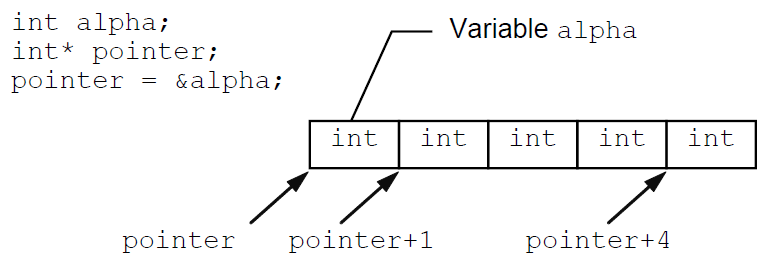
\includegraphics[height=2.5cm]{Bilder/ptr_add-subtraction.png}

			\textbf{Weitere Optionen:}\\
				Pointer funktioneren auch mit anderen Operatoren.\\
				\textbf{\textit{Vergleiche}} mit \verb|==, !=, <, >, >=, etc.| funktionieren bei Pointern desselben Typs.

	\subsection{Arrays}
			Arrays arbeiten mit Array-Index. In C beginnt dieser bei 0 und endet bei $n-1$:
			\begin{lstlisting}[language=C]
int alpha[5];  // Array "alpha" mit 5 El. vom Typ int
alpha[0] = 14; // 1. Element (Index 0) = 14
alpha[4] = 3;  // letztes Element (Index 4)
alpha[5] = 4;  // Bereichsueberschr.! -> undefined behaviour
			\end{lstlisting}
			\textbf{Memorymap:}\\
				\begin{minipage}{1\linewidth}
					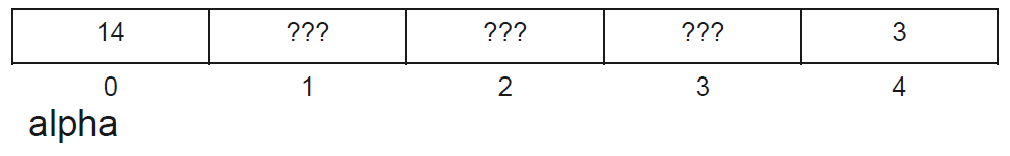
\includegraphics[width=0.5\linewidth]{Bilder/arr-mem-map.png}
				\end{minipage}

		\subsubsection{Initialisierungsvarianten}
			\begin{lstlisting}[language=C]
int a1[5] = {0, 8, 5, 1, 2};
int a2[5] = {1, 8};         //Index 1 bis 3 sind auf "0"
int a3[5] = {};             //Alle Elemente sind auf "0"
int a4[] = {12, 3, 2};      //Groesse anhand der Anz. Elemente => "[3]"
			\end{lstlisting}

		\subsubsection{Grösse eines Arrays}
			\verb|sizeof()| liefert bei Arrays die Grösse in \textbf{Bytes}\\
			Zur Bestimmung der Anzahl Elemente kann die Grösse des Arrays durch die Grösse eines Wertes geteilt werden:
			\begin{lstlisting}[language=C]
int main() {
	int arr[] = {4, 3, 2, 1};
	printf("arr hat %lu Elemente\n", sizeof(arr)/siezof(arr[0]));
	return 0;
}
			\end{lstlisting}

		\subsubsection{Mehrdimensionale Arrays}
			Arrays können auch als Matritzen verwendet werden, wobei der erste Wert der Zeilenindex und der zweite der Spaltenindex ist.\\
			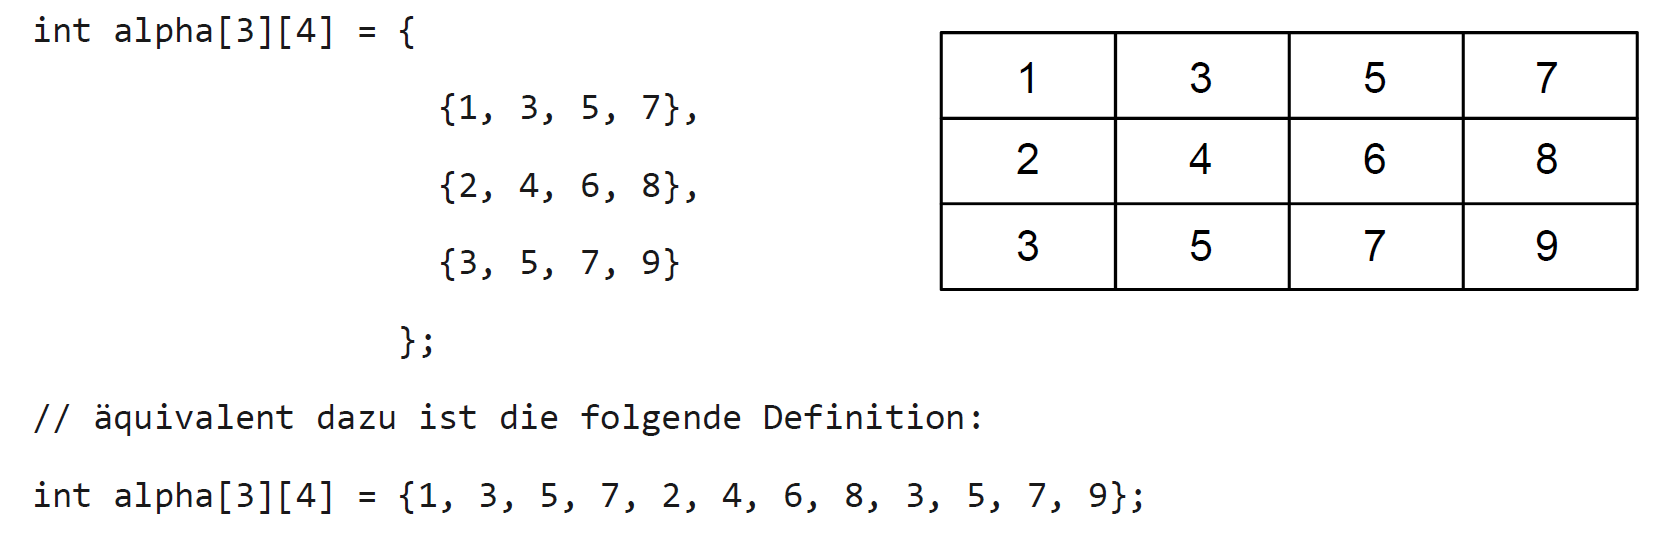
\includegraphics[height=3cm]{Bilder/arr_mehrdimensional.png}

		\subsubsection{char - Arrays}
			Ein String in C ist immer ein Array von Zeichen. (\verb|char| - Array).\\
			Ein String in C muss \textbf{immer} mit \verb|\0| abgeschlossen werden und braucht eine Stelle des Arrays!
			\begin{lstlisting}[language=C]
// Folgende Varianten sind gleichwertig:
char name[15] = {1, 2, 3, 4, 5, 0};
char name[15] = {'M', 'e', 'i' 'e', 'r', '\0'};
char name[15] = "Meier";
			\end{lstlisting}

		\subsubsection{Array mit Schleife durchlaufen (Bsp.)}
			\begin{lstlisting}[language=C]
enum{groesse = 5};
int alpha[groesse];

for(int i = 0; i < groesse; ++i)
	printf("%d \n", alpha[i]) // keine "{}", da nur eine Zeile
			\end{lstlisting}

		\subsubsection{Weitere Array-Regeln}
			\begin{itemize}
				\item Ein Array als Ganzes kann keine Werte annehmen, nur einzelne Elemente
				\item Die üblichen Operatoren können nicht auf Arrays angewendet werden
				\item Funktionen in C können \textbf{keine} Arrays als Aufrufparameter haben!
				\item Wird bei einem Funktionsaufruf ein Array als Parameter übergeben, wird das Array \textit{implizit zu einem Pointer auf das Element an Index 0 konvertiert}
				\item Der Name des Arrays kann als \textit{konst. Adresse} von Index 0 des Arrays verwendet werden: \verb|alpha[i] == *(alpha +i)| \\
				\textbf{Achtung!}
				\begin{itemize}
					\item Der Pointer \textbf{ptr} bewegt sich bei \textbf{ptr$+$n} immer um \textbf{n * sizeof(Typ)} Bytes!
					\item Wenn der Pointer über den Bereich hinauszeigt, ist das zwar legal, das Resultat ist aber undefiniert.
				\end{itemize}
				\item Zuweisung eines Arrays auf einen Pointer:\\
				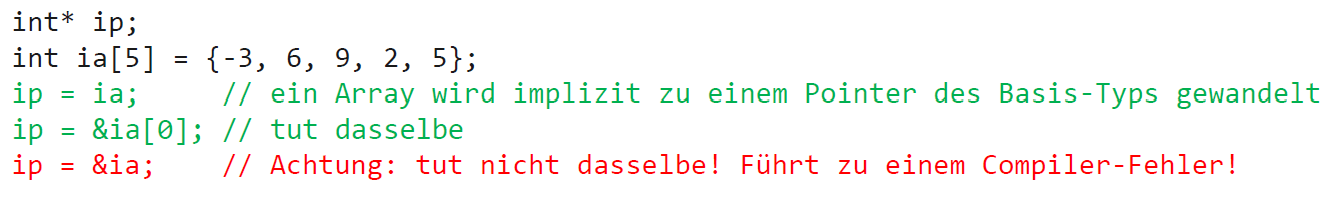
\includegraphics[height=2cm]{Bilder/arr-ptr-zuweisung.png}
				\item Benutzung eines Pointers im Array-Stil:\\
				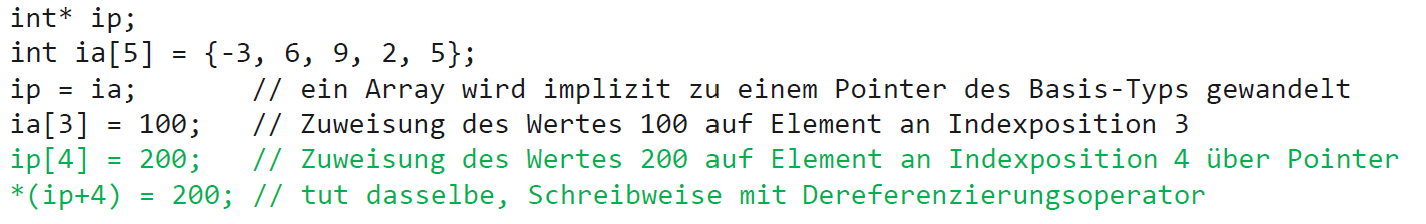
\includegraphics[height=2cm]{Bilder/ptr-im-arr-stil.png}	
			\end{itemize}

	\subsection{Structs}
		Arrays enthalten mehrere Elemente desselben Datentyps. Structs können im Gegensatz auch \textbf{unterschiedliche} Datentypen enthalten. \\
		\begin{minipage}{1\linewidth}
			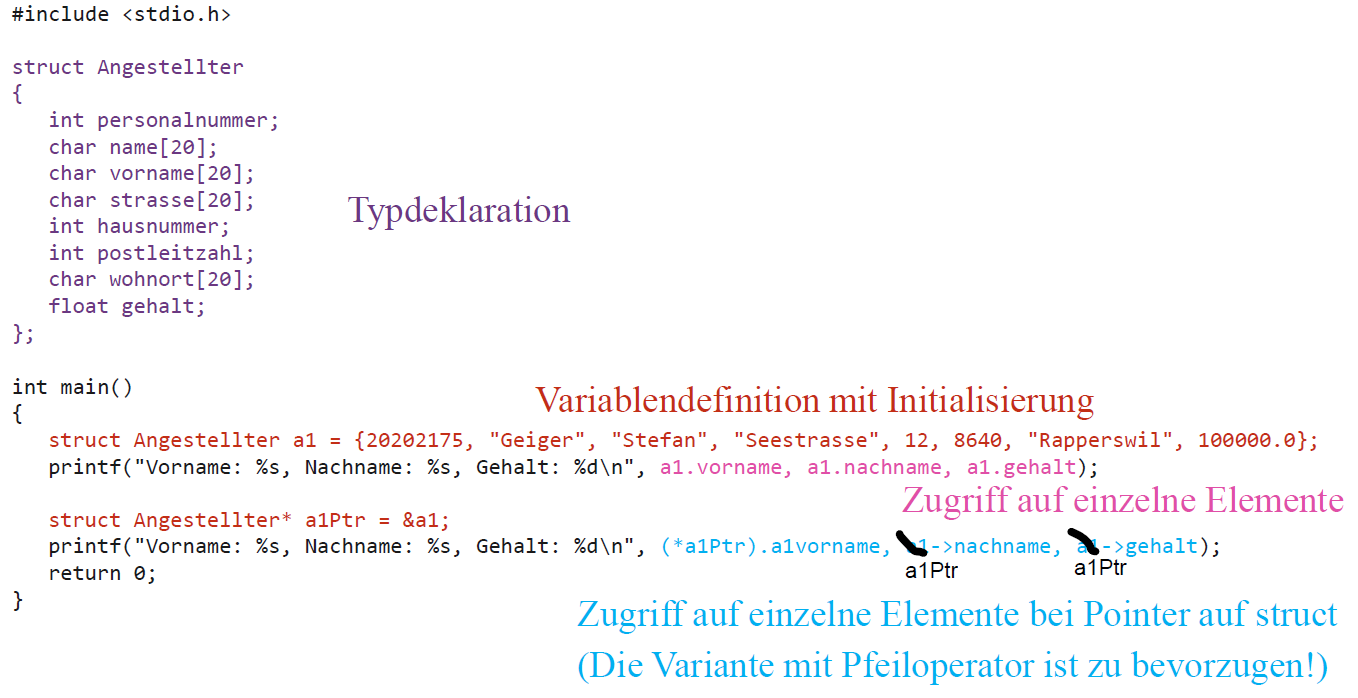
\includegraphics[width=0.9\linewidth]{Bilder/structs-bsp.png}
		\end{minipage}	

	\subsection{Strings und Speicher}
		Für alle Funktionen in diesem Kapitel: \verb|#include <string.h>|\\
		\textbf{Vorsicht:} Jeder Charakter im String benötigt je ein Byte, die \verb|'\0'|-Terminierung ein zusätzliches Byte
		\subsubsection{Strings kopieren}
			\begin{lstlisting}[language=C]
char* strcpy(char* dest, const char* src);

char* strncpy(char* dest, const char* src, size_t n);
			\end{lstlisting}
			\textbf{String copy}
				\begin{itemize}
					\item kopiert von \verb|src| nach \verb|dest|, inklusive \verb|'\0'| \\ (bei \verb|strncpy()| maximal n chars)
					\item return: \verb|dest|
					\item \verb|dest| muss bei \verb|strcpy()| auf einen genügend grossen Bereich zeigen\\ (Ansonsten werden Speicherbereiche nach \verb|dest| überschrieben)
				\end{itemize}

		\subsubsection{Strings zusammenfügen}
			\begin{lstlisting}[language=C]
char* strcat(char* dest, const char* src);

char* strncat(char* dest, const char* src, size_t n);
			\end{lstlisting}
			\textbf{String concatenate}
				\begin{itemize}
					\item hängt von \verb|src| nach \verb|dest| an, inklusive \verb|'\0'| \\
					(bei \verb|strncat()| maximal n chars) \\
					Das ursprüngliche \verb|'\0'| von \verb|dest| wird überschrieben 
					\item return: \verb|dest|
					\item \verb|dest| muss bei \verb|strcat()| auf einen genügend grossen Bereich zeigen\\ (Ansonsten werden Speicherbereiche nach \verb|dest| überschrieben)
				\end{itemize}

		\subsubsection{Strings vergleichen}
			\begin{lstlisting}[language=C]
char* strcmp(const char* s1, const char* s2);

char* strncmp(const char* s1, const char* s2, size_t n);
			\end{lstlisting}
			\textbf{String compare}
				\begin{itemize}
					\item vergleicht die beiden Strings, auf die \verb|s1| und \verb|s2| zeigen,\\
					bei \verb|strncmp()| nur die ersten n char's
					\item return:
					\begin{itemize}
						\item $<0$ : *s1 ist lexikographisch kleiner als *s2
						\item $==0$: *s1 und *s2 sind gleich
						\item $>0$ : *s1 ist lexikographisch grösser als *s2
					\end{itemize}
				\end{itemize}
		\subsubsection{Stringlänge bestimmen}
			\begin{lstlisting}[language=C]
size_t strlen(const char* s);
			\end{lstlisting}
			\textbf{String length}
				\begin{itemize}
					\item bestimmt die Länge des Strings s, d.h. die Anazhl char's. \verb|'\0'| wird nicht mitgezählt 
					\item return: Länge des Strings
				\end{itemize}
		\subsubsection{Speicher bearbeiten}
			\begin{itemize}
				\item Aufrufparams sind vom Typ \verb|void*| statt \verb|char*|
				\item Die \textbf{mem}-Funktionen arbeiten byteweise
				\item Das \verb|'\0'|-Zeichen wird nicht speziell behandelt wie bei den \textbf{str}-Funktionen
				\item Die Bufferlänge muss als Parameter übergeben werden
			\end{itemize}
			\begin{lstlisting}[language=C]
//Speicherbereich kopieren (ohne Ueberlappung!)
void* memcpy(void* dest, const void* src, size_t n);

//Speicherbereich verschieben
void* memmove(void* dest, const void* src, size_t n);

//Speicherbereiche vergleichen
int memcmp(const void* s1, const void* s2, size_t n);

//Erstes Auftreten von Zeichen c in Bereich s suchen
void* memchr(cont void* s, int c, size_t n);

//Speicherbereich mit Wert belegen
void* memset(void* s, int c, size_t n);
			\end{lstlisting}

	\subsection{Static}
		\underline{\textbf{\textit{static}-Funktionen}}
			\begin{itemize}
				\item \verb|static|-Funktionen sind nur in der Compile-Unit, in welcher sie definiert sind, sichtbar
				\item Alle Funktionen, welche von aussen nicht sichtbar sein müssen, sollten deshalb als \verb|static| definiert werden
				\item Ein versuchter Zugriff auf statische Elemente von einer weiteren Datei ergibt einen Linkerfehler
				\item \textbf{Alle Funktionen \textit{static} definieren, welche keine Schnittstelle nach aussen bilden!}
			\end{itemize}
		
		\underline{\textbf{\textit{static}-Variablen}}
			\begin{itemize}
				\item Globale Variablen
				\begin{itemize}
					\item Analog zu den Funktionen: nur am Definitionsort gültig
				\end{itemize}
				\item Lokale Variablen
				\begin{itemize}
					\item \textbf{Achtung: Komplett andere Bedeutung desselben Schlüsselwortes!}
					\item Lokale \textit{static}-Variablen haben eine Lebensdauer wie eine globale Variable. Dadurch bleibt der Wert der lokalen Variable erhalten, auch wenn die Funktion verlassen wird.\\
					($\rightarrow$ Gleiches Verhalten wie globale Variable, abgesehen von der \textit{Sichtbarkeit})
					\item Werden automatisch mit 0 initialisiert
					\item $\rightarrow$ Kompromiss zwischen gloabler und lokaler Variable
				\end{itemize}
			\end{itemize}

	\subsection{Iterativ vs. Rekursiv}
		\begin{minipage}{0.49\linewidth}
			Iterativ:\\
			$0! = 1$ \\
			$n! = 1 \cdot 2 \cdot ... \cdot (n-1) \cdot n$
			\begin{lstlisting}[language=C]
unsigned long
faku(unsigned int n){
	unsigned long fak = 1UL;
	for(unsigned int i = 2; i <= n; ++i)
		fak = fak * i;
	return fak;
}
			\end{lstlisting}
		\end{minipage}
		\hfill
		\begin{minipage}{0.49\linewidth}
			Rekursiv:\\
			$0! = 1$ \\
			$n! = $\textbf{(n-1)!}$ \cdot n$
			\begin{lstlisting}[language=C]
unsigned long
faku(unsigned int n){
	if(n > 1)
		return n * faku(n-1);
	else
		return 1UL;
}
				\end{lstlisting}
		\end{minipage}
	
	\subsection{Präprozessor}
		\begin{tabular}{ll}
			\verb|#define ALT NEU|  & Ersetzt ALT durch NEU \\
			\verb|#include| $"$Datei$"$ & Fügt Inhalt aus Datei an die aktuelle Position \\
			\verb|#include| $<$Datei$>$ & Gleich wie oben \\
			\verb|#ifdef Marke ... #endif| & Prüt, ob Marke definiert ist \\
			\verb|#ifndef Marke ... #endif| & Prüt, ob Marke nicht definiert ist \\
			\verb|#error(Nachricht)| & Bricht den Compile-Vorgang ab \\ 
		\end{tabular}

		\subsubsection{Beispiel}
			\begin{lstlisting}[language=C]
#include <stdio.h>

#ifndef __cplusplus
	#error Ich brauche keinen C++-Compiler
#endif

#ifdef __APPLE_
	#error Ich mag keine Aepfel
#endif

#ifdef __WIND32__
	#error Ich mag kein Windows
#endif

int main(){
	printf("Ich bin sehr waehlerisch\n");
	return 0;
}
			\end{lstlisting}

	\subsection{Trivia}
		\subsubsection{Funktionsprototypen}
			Funktionsprototypen legen die Schnittstelle ener Funktion fest.\\
			Sie sind zwingend erforderlich, wenn Funktionen vor ihrer Definition aufgerufen werden.
		
		\subsubsection{Call-by-Reference vs. Call-by-Value}
			\begin{tabular}{|ll|l|}
				\hline
				\textbf{Call-by-Reference:} & & \textbf{Call-by-Value:}\\
				\hline
				An eine zu rufende Funktion werden Pointer auf & & An eine zu rufende Funktion werden \\
				Variablen übergeben, an denen Werte stehen können & & Werte übergeben \\
				\verb|int s1 = 3;| & & \verb|int summe = add(3,7);|\\
				\verb|int s2 = 7;| & & \\
				\verb|int summe;| & & \\
				\verb|add(&s1, &s2, &summe);| & & \\
				\hline
			\end{tabular}
			
		\subsubsection{C-Compiler}
			Der C-Compiler überprüft den Quelltext auf syntaktische Korrektheit.\\
			Zusätzlich übersetzt er den Quelltext in Maschinencode für eine bestimmte Zielplattform.

		\subsubsection{Gleitpunktzahlen}
			Eine Gleitpunkzahl ist ein Datentyp in Exponentialdarstellung, bestehend aus Vorzeichen, Mantisse und Exponent.
			Diese drei Bestandteile werden im Computer separat im Speicher binär dargestellt, gem. Standard IEEE 754.
			In C gibt es hierfür die Datentypen \verb|float| und \verb|double|.

			\textbf{Vorteil:} sehr grosser Wertebereich von $-\infty$ bis $\infty$\\
			\textbf{Nachteil:} Rundungsfehler treten zwangsläufig auf und sind sehr schwer abschätzbar.
			Sie sollten daher nie auf Gleichheit geprüft werden!
		
	\subsection{Code-Snippets}
		\subsubsection{Array und Pointer 1}
			\begin{lstlisting}[language=C]
#include <stdio.h>

int main(){
	enum{array_size = 6};
	int test[array_size] = {1,2,3,4,5,6};
	for(int i =0; i<array_size; ++i)
		printf("Element %u: %i\n", i, test[i]);
	
	printf("Groesster: %d", *findAbsMax(test, array_size));
	return 0;
}
			\end{lstlisting}
			Main-Funktion zum Finden eines \textbf{betragsmässig} grössten Wertes innerhalb eines Arrays.

			\begin{lstlisting}[language=C]
int* findAbsMax(int* arr, size_t size){
	int* max_ptr = &arr[0];
	for(size_t i = 0; i < size; ++i){
		if((arr[i] >=0 && *max_ptr >=0 && arr[i] > *max_ptr)
		|| (arr[i] <=0 && *max_ptr <=0 && arr[i] < *max_ptr)
		|| (arr[i] >=0 && *max_ptr <=0 && arr[i] > *max_ptr * -1)
		|| (arr[i] <=0 && *max_ptr >=0 && arr[i] * -1 > *max_ptr))
			max_ptr = &arr[i];
	}
	return max_ptr;
}
			\end{lstlisting}
			%\par\noindent\rule{\linewidth}{0.2pt} %war gedacht als Trenner, ist aber durch Formatierung überflüssig
		
		\subsubsection{Array und Pointer 2}
			Programm liest Wert um Wert ein und gibt sie wieder zurück. \verb|init| in Pointer-Schreibweise, \verb|ausgabe| in Array-Schreibweise.
			\begin{lstlisting}[language=C]
#include <stdio.h>
enum{groesse = 3};

void init(int* alpha, int dim){ //alpha in Pointer-Schreibweise
	for(int i = 0; i < dim, ++i){
		printf("Eingabe Wert mit Index %d von arr:", i);
		scanf("%d", alpha++);
	}
}

void ausgabe(const int alpha[], int dim){ //alpha in Array-Schreibweise
	for(int i = 0; i < dim; ++i)
		printf("arr[%d] hat Wert: %d\n", i, alpha[i])
}

int main(void){
	int arr[groesse];
	init(arr, sizeof(arr)/sizeof(arr[0]));
	ausgabe(arr, sizeof(arr)/sizeof(arr[0]));
	return 0;
}
			\end{lstlisting}

		\subsubsection{Bitweise Zahl ausgeben}
			Funktion gibt die Zahl bitweise aus, beginnend mit MSB\\
			In diesem Fall 1000'0000
			\begin{lstlisting}[language=C]
unsigned char x = 128;
for(int i = 0; i < 8; i++){
	int bitValue = 1 & x;
	printf("%d", bitValue);
	x = x >> 1;
}
return 0;
			\end{lstlisting}

		\subsubsection{Drehmoment berechnen}
			\textbf{Programm:}
			\begin{lstlisting}[language=C]
#include<stdio.h>
int main(){
	float kraft;
	float abstand;
	printf("Kraft F in N: ");
	scanf("%f", &kraft);
	printf("Abstand s in m: ");
	scanf("%f", &abstand);
	if(abstand < 0.0f){
		printf("Fehler: Abstand ist negativ!");
		return -1;
	}
	else{
		printf("Das Drehmoment ist: %f Nm\n", kraft*abstand);
		return 0;
	}
}
			\end{lstlisting}

			\textbf{Ausgabe:}\\
			\verb|Kraft F in N:| -17\\
			\verb|Abstand s in m: | 0.5\\
			\verb|Das Drehmoment ist: -8.500 Nm|

		\subsubsection{Pointer \& Memorymaps}
			\begin{lstlisting}[language=C]
#include <stdio.h>
void geheim(double* p, double z){
	z  = 2.0 * z;
	*p = z;
}

int main(void){
	double u = 5.0;
	double v = 7.0;
	geheim(&u, v);
	printf("u= %f, v= %f\n", u, v);
	return 0;
}
			\end{lstlisting}
			
			\textbf{Memorymap kurz vor \textit{geheim}-Aufruf}\\
				\begin{minipage}{0.9\linewidth}
					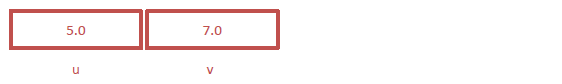
\includegraphics[width=1\linewidth]{Bilder/memmap-vor-geheim.png}
				\end{minipage}

			\textbf{Memorymap kurz nach \textit{geheim}-Aufruf}\\
				\begin{minipage}{0.9\linewidth}
					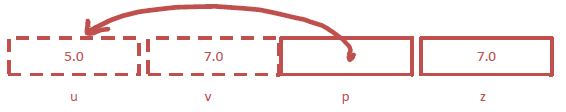
\includegraphics[width=1\linewidth]{Bilder/memmap-aufruf-geheim.png}
				\end{minipage}

			\textbf{Memorymap kurz vor \textit{geheim}-Verlassen}\\
				\begin{minipage}{0.9\linewidth}
					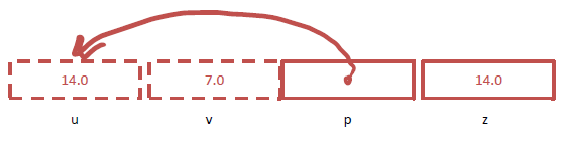
\includegraphics[width=1\linewidth]{Bilder/memmap-vor-verlassen.png}
				\end{minipage}

			\textbf{Memorymap kurz nach \textit{geheim}-Verlassen}\\
				\begin{minipage}{0.9\linewidth}
					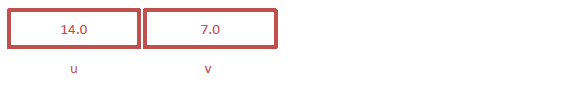
\includegraphics[width=1\linewidth]{Bilder/memmap-nach-verlassen.png}
				\end{minipage}

			\textbf{Ausgabe des Programms:}\\
				\verb*|u= 14.0, v= 7.0<newline>|

		\subsubsection{Grösster gemeinsamer Teiler}
			\begin{minipage}{0.45\linewidth}
				\begin{lstlisting}[language=C]
typedef unsigned int uint;
uint func(uint m, uint n){
	uint r;
	uint h;
	do{
		if(m<n){
			h=m;
			m=n;
			n=h;
		}
		r=m%n;
		if(r!=0){
			m=n;
			n=r;
		}
	}while(r!=0);
	return n;
}
				\end{lstlisting}
			\end{minipage}
			\hfill
			\begin{minipage}{0.5\linewidth}
				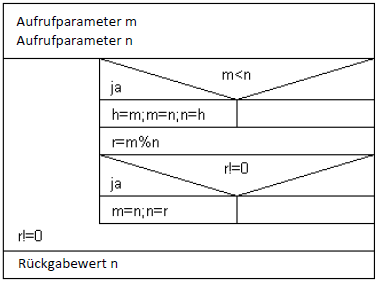
\includegraphics[width=1\linewidth]{Bilder/snippets-ggt.png}
			\end{minipage}